\documentclass[12pt,a4paper]{scrartcl}

\usepackage{amsmath}
\usepackage{amssymb}

\usepackage{tikz}
\usepackage{pgfplots}
\usetikzlibrary{math}
\usepgfplotslibrary{groupplots}

\begin{document}
\author{Pavankumar Deshpande, Dmitrii Panichev, Paul Kröpke, Daniel Biskup}
\title{Foundations of Audio Signal Processing:}
\subtitle{Exercise sheet 9}
\maketitle

\section*{Exercise 9.1}
\subsection*{(a)}

\begin{figure}[!htb]
\centering
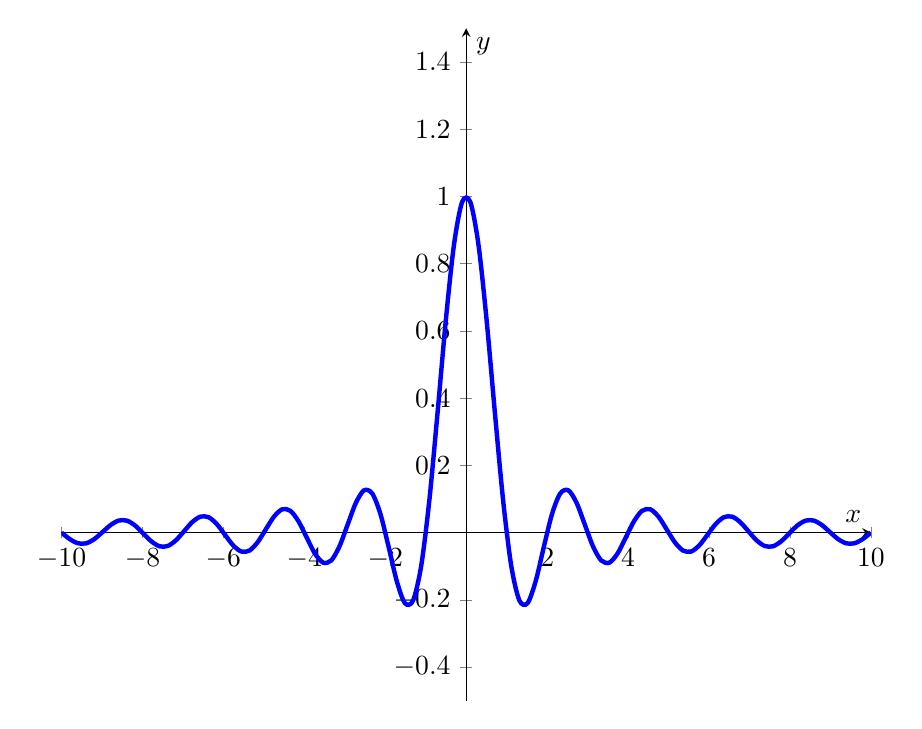
\begin{tikzpicture}
\begin{axis}[
  xmin=-10,
  xmax=10,
  ymin=-0.5,
  ymax=1.5,
  xlabel=$x$,
  ylabel=$y$,
  axis lines=center,
  scale=1.5,
  transform shape,
  >=stealth
]
  \addplot[
    domain=-10:10,
    blue,
    ultra thick,
    samples=100,
  ] plot[smooth] {sin(deg(pi*x))/(pi*x)};
\end{axis}
\end{tikzpicture}
\caption{Plot of sinc(x).}
\end{figure}

\begin{figure}
\centering
\begin{tikzpicture}
\pgfmathdeclarefunction{p}{1}{%
  \pgfmathparse{%
            abs(#1)<0.001 ? 1 : sin(deg(pi*(#1)))/(pi*(#1))%
            }%
        }
\begin{axis}[
  domain = -10:10,
  samples = 21,
  xmin=-10,
  xmax=10,
  ymin=-0.5,
  ymax=1.5,
  xlabel=$x$,
  ylabel=$y$,
  axis lines=center,
  scale=1.5,
  transform shape,
  >=stealth
]
\addplot+[
  domain=-10:10,
  samples=21,
  ycomb,
  black,
  thick]  {p(x)};
\end{axis}
\end{tikzpicture}
\caption{Plot of sampled sinc(x) with T=1.}
\end{figure}

\newpage
\text{Sampling rate is $\frac{1}{T}=\frac{1}{1}=1$Hz}

\begin{figure}
\centering
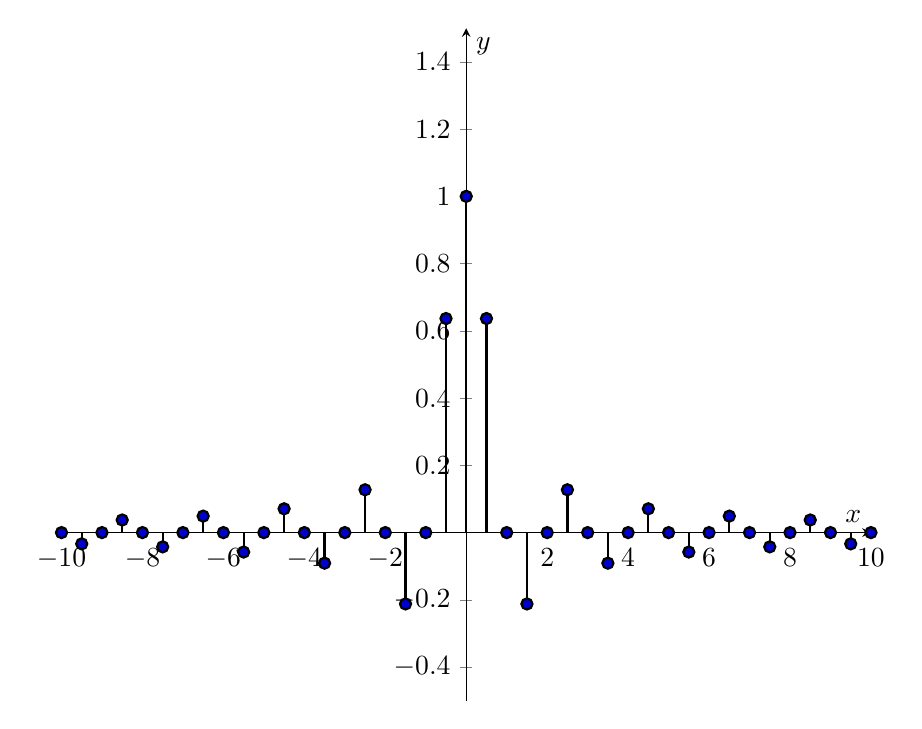
\begin{tikzpicture}
\pgfmathdeclarefunction{p}{1}{%
  \pgfmathparse{%
            abs(#1)<0.001 ? 1 : sin(deg(pi*(#1)))/(pi*(#1))%
            }%
        }
\begin{axis}[
  domain = -10:10,
  samples = 41,
  xmin=-10,
  xmax=10,
  ymin=-0.5,
  ymax=1.5,
  xlabel=$x$,
  ylabel=$y$,
  axis lines=center,
  scale=1.5,
  transform shape,
  >=stealth
]
\addplot+[
  domain=-10:10,
  samples=41,
  ycomb,
  black,
  thick]  {p(x)};
\end{axis}
\end{tikzpicture}
\caption{Plot of sampled sinc(x) with T=0.5.}
\end{figure}

\newpage
\text{Sampling rate is $\frac{1}{T}=\frac{1}{0.5}=2$Hz}

\begin{figure}
\centering
\begin{tikzpicture}
\pgfmathdeclarefunction{p}{1}{%
  \pgfmathparse{%
            abs(#1)<0.001 ? 1 : sin(deg(pi*(#1)))/(pi*(#1))%
            }%
        }
\begin{axis}[
  domain = -10:10,
  samples = 11,
  xmin=-10,
  xmax=10,
  ymin=-0.5,
  ymax=1.5,
  xlabel=$x$,
  ylabel=$y$,
  axis lines=center,
  scale=1.5,
  transform shape,
  >=stealth
]
\addplot+[
  domain=-10:10,
  samples=11,
  ycomb,
  black,
  thick]  {p(x)};
\end{axis}
\end{tikzpicture}
\caption{Plot of sampled sinc(x) with T=2.}
\end{figure}

\newpage
\text{Sampling rate is $\frac{1}{T}=\frac{1}{2}=0.5$Hz}

\subsection*{(b)}
\text{Fourier transform for $f(t)=sinc(t)$ is $\widehat{f}(w)=rect(w)$}\\

\begin{equation}
  rect(w)=
  \begin{cases}
     0, & \text{if}\ |w|> \frac{1}{2} \\
     1/2, & \text{if}\ |w| =  \frac{1}{2} \\
     1, & \text{if}\ |w| <  \frac{1}{2} \\
  \end{cases}
\end{equation}

\text{By definition, sinc(t) is 0.5-bandlimited, and 0.5 is such smallest $\Omega$}

\subsection*{(c)}

\text{By Shannon's theorem, an $\Omega$-bandlimited signal needs to be sampled with rate $ > 2\Omega$ in order to be}
\text{fully reconstructible. In case of $sinc$, sampling rate should be $> 2*0.5 = 1$ Hz}\\
\text{For $T=1$ sampling rate $\Omega = \frac{1}{T} = 1$Hz is not $> 1$Hz. Thus, signal is not fully reconstructible}\\
\text{For $T=\frac{1}{2}$  sampling rate $\Omega = \frac{1}{T} = 2$Hz $> 1$Hz. Thus, signal is fully reconstructible}\\
\text{For $T=2$  sampling rate $\Omega = \frac{1}{T} = 0.5$Hz $< 1$Hz. Thus, signal is not fully reconstructible}\\

\newpage
\section*{Exercise 9.2}
\subsection*{(a)}

\begin{equation}
(\uparrow M \circ T^k)[x](n) =
\begin{cases}
  x(\frac{n}{M} - k), & \mbox{if } M\vert n\\
  0, & \mbox{otherwise}
\end{cases}
\end{equation}

\begin{equation}
(T^k \circ \uparrow M)[x](n) =
\begin{cases}
  x(\frac{n-k}{M}), & \mbox{if } M\vert n-k\\
  0, & \mbox{otherwise}
\end{cases}
\end{equation}

\text{Since $(\uparrow M \circ T^k)[x](n) \neq (T^k \circ \uparrow M)[x](n)$, upsampling operator is not time invariant}

\subsection*{(b)}
\begin{equation}
(T^k \circ E_\omega)[x](n) = e^{-2\pi iwn} x(n-k)
\end{equation}

\begin{equation}
( E_\omega \circ T^k)[x](n) =e^{-2\pi iw(n-k)}x(n-k)
\end{equation}

\text{Since $\forall w \neq 0$, $(\uparrow M \circ T^k)[x](n) \neq (T^k \circ \uparrow M)[x](n)$, frequency shift operator is not time invariant}\\

\end{document}